\subsection{}

\begin{definition}
    \emph{The equilibrium point} is where the supply and demand curves intersect.
    Price of the product is the variable that brings the market to equilibrium.\\
    $P^*$ and $Q^*$ are the equilibrium price and quantity.\\
\end{definition}
\begin{figure}[h!]
    \centering
    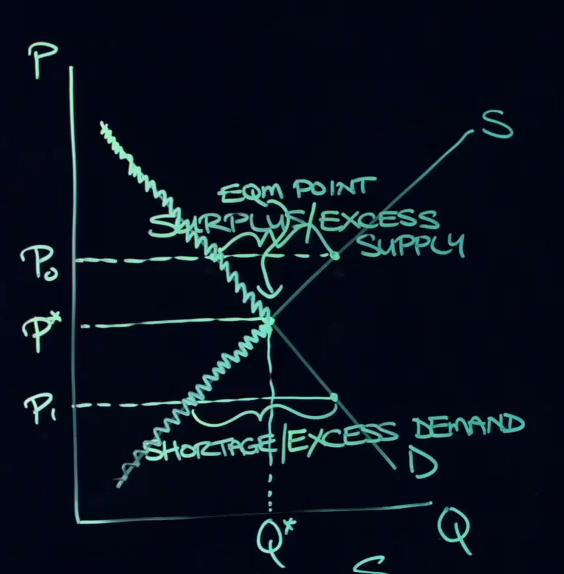
\includegraphics[]{Chapter3/DemandSupplyGraph.png}
    \caption{Demand Supply Graph}
\end{figure}
If prices raise above the equilibrium price, there will be a surplus in supply. If prices fall below the equilibrium price, there will be a shortage.\\
The invisible hand of the market that guides consumers and producers will bring the market back to equilibrium.\\
The short-side (left of $Q^*$) of the market decides what happens.\\
\emph{Laissez faire} is the idea that the government should not interfere with the market.\\
There are 9 different cases of supply and demand shifts.\\
\begin{figure}
    \centering
    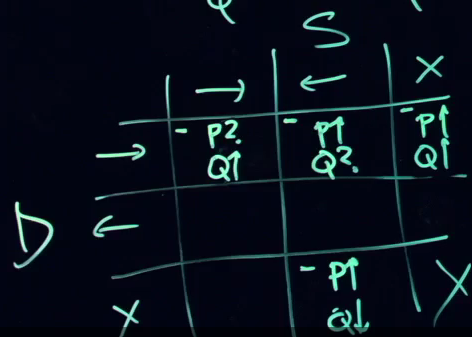
\includegraphics[]{Chapter3/DemandSupplyShifts.png}
    \caption{Demand Supply Scenarios}
\end{figure}
In some scenarios, for example if supply and demand both shift right, the equilibrium price is ambiguous.
The price depends on how much demand or supply shifts right.\\
\begin{figure}[H]
    \centering
    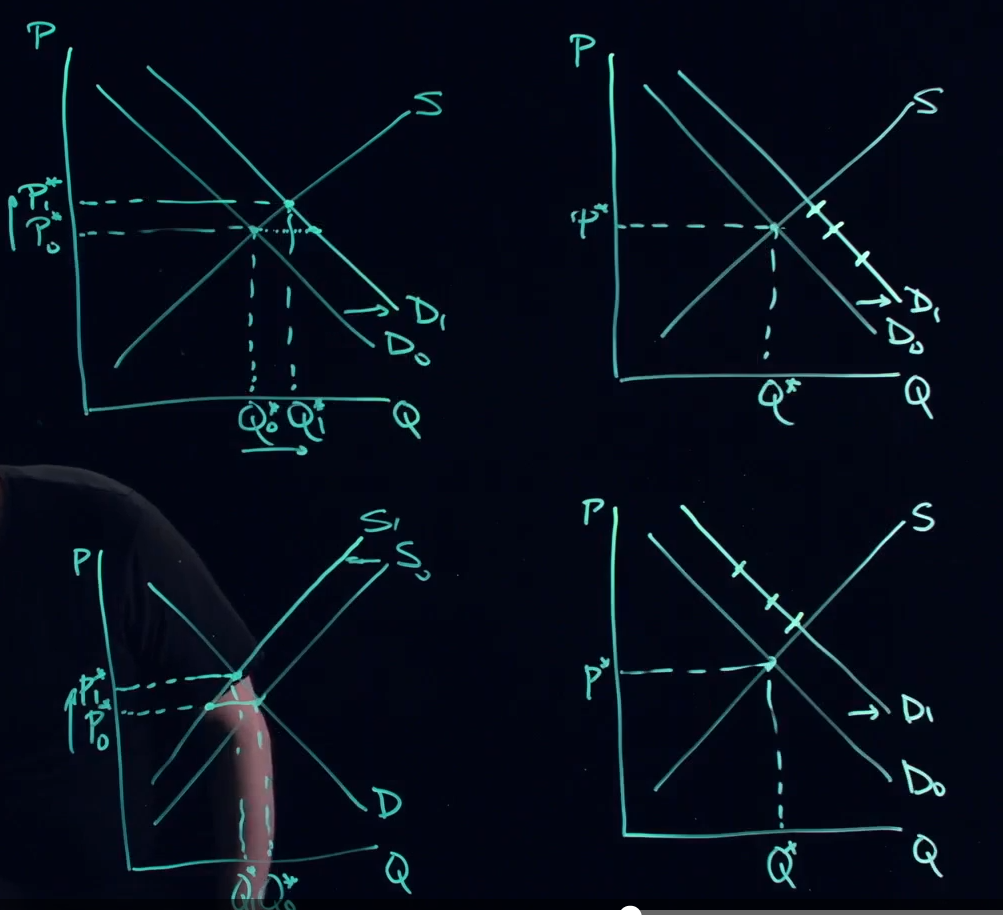
\includegraphics[scale=0.5]{Chapter3/DemandSupplyShiftGraphs.png}
    \caption{Demand Supply Scenarios}
\end{figure}